\documentclass[aspectratio=169]{beamer}

\usetheme{Madrid}
\usecolortheme{default}

\usepackage{amsmath}
\usepackage{booktabs}
\usepackage{hyperref}
\usepackage{graphicx}

% ── Metadata ──────────────────────────────────────────────────────────────────
\title[Polymarket SPY Signal]{Polymarket SPY\\Directional Signal Strategy}
\subtitle{Using Prediction Markets to Trade the S\&P 500}
\author{}
\institute{}
\date{April 24, 2026}

% ══════════════════════════════════════════════════════════════════════════════
\begin{document}

% ── Title slide ───────────────────────────────────────────────────────────────
\begin{frame}
  \titlepage
\end{frame}

% ── 1 · The Market ────────────────────────────────────────────────────────────
\begin{frame}{The Market}

  \begin{block}{Polymarket — SPY Up or Down?}
    A \textbf{daily binary market} that resolves \texttt{YES} if the official
    SPY close (Pyth Network price feed) is \emph{higher} than the previous
    trading day's close.
  \end{block}

  \vspace{0.4em}

  \begin{columns}[T]
    \column{0.48\textwidth}
      \textbf{Key mechanics}
      \begin{itemize}
        \item New contract every trading day
        \item Two outcome tokens: \texttt{Up} / \texttt{Down}
      \end{itemize}

    \column{0.48\textwidth}
      \textbf{Settlement}
      \begin{itemize}
        \item Price source: \textbf{Pyth Network} oracle
        \item Market opens: 09:30 ET (15:30 FR)
        \item Resolved at NYSE close: 16:00 ET (22:00 FR)
        \item Trading window: 6.5 hours of liquidity
      \end{itemize}
  \end{columns}

\end{frame}

% ── 2 · Example: April 21 ─────────────────────────────────────────────────────
\begin{frame}{Example — April 21, 2026}
      \center
      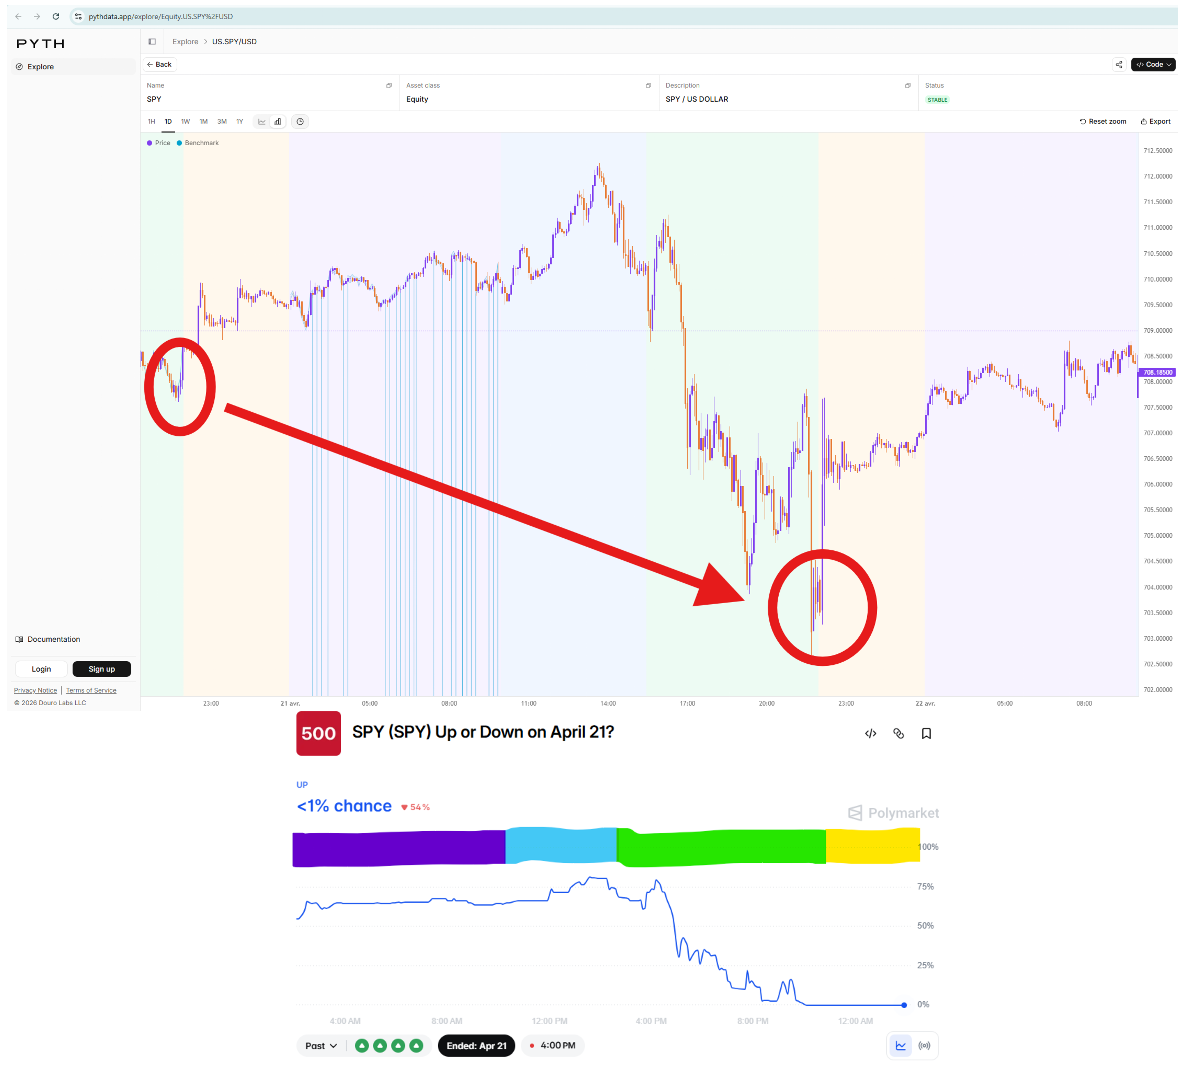
\includegraphics[height=0.8\textheight]{PriceExample2.png}
\end{frame}

% ── 3 · Strategy Ideas ────────────────────────────────────────────────────────
\begin{frame}{Strategy Ideas}

  \begin{block}{1 · Base rate: SPY almost always goes up}
    \begin{itemize}
      \item Check historical \textbf{win rate} of daily Up moves
      \item Measure average gain on up days vs.\ average loss on down days
      \item Apply \textbf{Kelly criterion} (2 outcomes with expected returns and a probability)
    \end{itemize}
  \end{block}

  \begin{block}{2 · Hedging with SPY}
    \begin{itemize}
      \item Buy \texttt{Up} token on Polymarket + short SPY ETF (or vice-versa)
      \item Delta-neutral position: profit from mispricing
    \end{itemize}
  \end{block}

  \begin{block}{3 · Predict SPY direction from $P(\text{Up})$}
    \begin{itemize}
      \item Use Polymarket probability as a real-time signal: $\text{signal} = 2 P(\text{Up}) - 1$
    \end{itemize}
  \end{block}

\end{frame}

% ══════════════════════════════════════════════════════════════════════════════
\end{document}
